\documentclass[../main.tex, class=article]{subfiles}
\graphicspath{{./images}}




\begin{document}
\subsection{Funzioni tipo potenza}\label{sec:funzioni_tipo_potenza}
Una funzione tipo potenza è una funzione nella forma:
\begin{equation*}
        f(x) = x^n
\end{equation*}

dove $ x^n = \underbrace{x*x*x*x*x\ldots*x}_\text{n volte} $.


\begin{procol}{2}

n pari:
\begin{itemize}
        \item $ dom(f) = \mathbb{R} $
        \item $ Im(f) = [) $
\end{itemize}
        
\switchcolumn\

n dispari:
\begin{itemize}
        \item $ dom(f) = \mathbb{R} $
        \item $ Im(f) = \mathbb{R} $
        \item \textit{strettamente costante}
        \item  a 
        \item $f(-x) = -f(x)$
        \item $ f $ è dispari.
\end{itemize}

\end{procol}







\todo{Aggiungere lezione 4}

\subsection{Proprietà dell'esponenziale e del logaritmo}

\begin{paracol}{2}
Alcune proprietà degli esponenziali:
\begin{itemize}
        \item $a^{x+y} = a^x * a^y$
        \item $a^{x*b} = (a^x)^b$
        \item $a^{-x} = (a^x)^{-1} = \frac{1}{a^x}$
        \item $a^0 = 1$
        \item $a^1 = a$
\end{itemize}

\switchcolumn

Alcune proprietà dei logaritmi: 
\begin{itemize}
        \item $\log_a(x*y) = \log_a(x) + \log_a(y)$
        \item $\log_a(x^b) = b * \log_a(x) $
        \item $\log_a(\frac{1}{x}) = \log_a(x^{-1}) = -\log_a(x) $
        \item $\log_a(1) = 0$
        \item $\log_a(a) = 1$
\end{itemize}
\end{paracol}

\bigskip

$ \log(x) $ è stato introdotto come funzione inversa dell'esponenziale $ a^x $ infatti dire: $ \log a(y) $ vuol dire trovare $ x $ tale
che:
\begin{align*}
       \log_a(y) = x \Leftrightarrow a^x = y \\
       \log_2(4) = x \Leftrightarrow 2^x = 4
\end{align*}
Una base $ a $ particolare è la $ e $ ovvero \textbf{Numero di Nepero}~\ref{sec:numero_di_nepero}, in particolare:
\begin{equation*}
        \log_e(x) = \ln(x)
\end{equation*}
Dove $ \ln $ è il \textbf{logaritmo naturale}



$ \log_a(x) = \log_b * \log_a(b)$ 

Alcune propiretà dell'inversione sono:
\begin{itemize}
        \item $a^{\log_a(x)} = x$
\end{itemize}
\todo{Proprietà mancante 9:33}



\subsection{Funzioni trigonometriche}

$ \alpha $ misura $ x $ radianti se  $ x $ è la lunghezza dell'arco di cerchio presente dentro l'angolo sapendo che la circonferenza è $ \boxed{2\pi}$.
\begin{figure}[H]
  	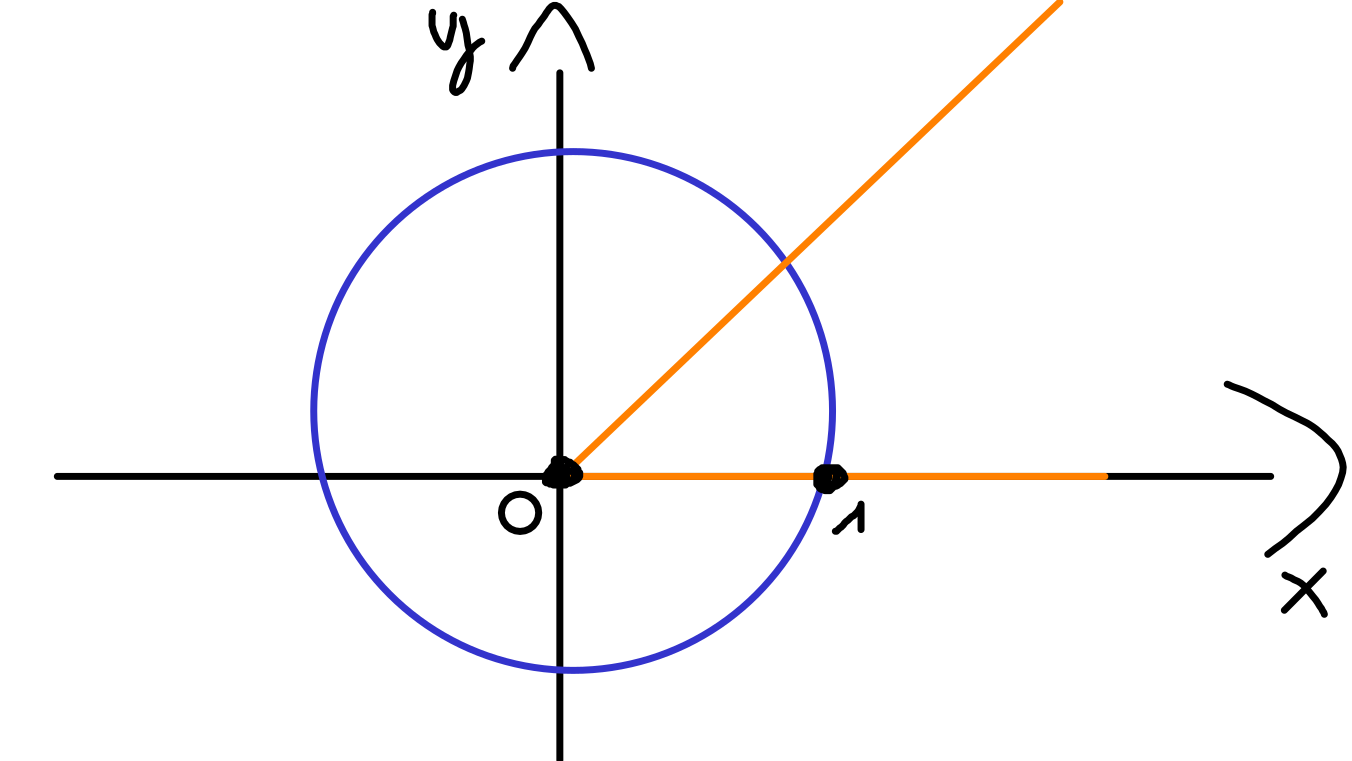
\includegraphics[width=\linewidth]{funzione_goniometrica.png}
  	\caption{}
        \label{fig:funzione_trigonometrica}
\end{figure}



\begin{exmp}
        Per esempio un angolo retto che è $ \dfrac{1}{4} $ della circonferenza sarà $\dfrac{2\pi}{4} = \dfrac{\pi}{2}$ 
\end{exmp}

In generale un angolo in radianti è:
\begin{equation*}
       \frac{\mbox{Angolo in gradi sessadecimali}}{360} * 2\pi 
\end{equation*}
\todo{Aggiungere 9:45 esepi seno coseno tangente}

\begin{itemize}
        \item $ tg(x) = \dfrac{\sin(x)}{\cos(x)} $
        \item $ cotg(x) = \dfrac{\cos(x)}{\sin(x)} $
        \item geometricamente noto che $PH \le PA \le QA $ e $ \sin(x) $
\end{itemize}




\end{document}
